% Anastasios Gerasis: completed analysis of the frozen confirmation results.
\subsection{Uncertainty and Exploratory Associations}
\label{sec:extended-analysis}
\paragraph{Paired uncertainty.}
We resample the 36 confirmation landmarks as paired units, retaining each landmark's method and reference scores together. With 100,000 bootstrap replicates and seed 20261126, all six pointwise 95\% percentile intervals for mean differences include zero (Table~\ref{tab:bootstrap}). None of six exact two-sided win/loss sign tests survives Holm correction. Tied pairs are excluded from those tests. These findings do not establish equivalence. Resampling this deliberately selected cohort describes uncertainty conditional on its composition and does not certify coverage for the 396-landmark population.

\begin{table*}[t]
\caption{Paired mean differences and bootstrap uncertainty on 36 confirmation landmarks. Negative favors the structured rule. W/T/L denotes improved/tied/worsened landmarks. Intervals are pointwise, not simultaneous. Every interval includes zero.}
\label{tab:bootstrap}
\centering
\begin{tabular}{llrrr}
\toprule
Rule & Reference & Mean $\Delta$ & Pointwise 95\% interval & W/T/L\\
\midrule
H1 & Original & $+0.2164$ & $[-0.7849, +1.4040]$ & 21/0/15\\
H1 & Scalar & $-0.6224$ & $[-1.5247, +0.1813]$ & 23/0/13\\
H2 & Original & $+0.8427$ & $[-0.1018, +2.2123]$ & 20/0/16\\
H2 & Scalar & $+0.0039$ & $[-0.7783, +0.6863]$ & 13/0/23\\
H3 & Original & $+0.4834$ & $[-0.3451, +1.6351]$ & 22/0/14\\
H3 & Scalar & $-0.3553$ & $[-0.9500, +0.0112]$ & 2/33/1\\
\bottomrule
\end{tabular}

\end{table*}

\begin{figure*}[t]
\centering
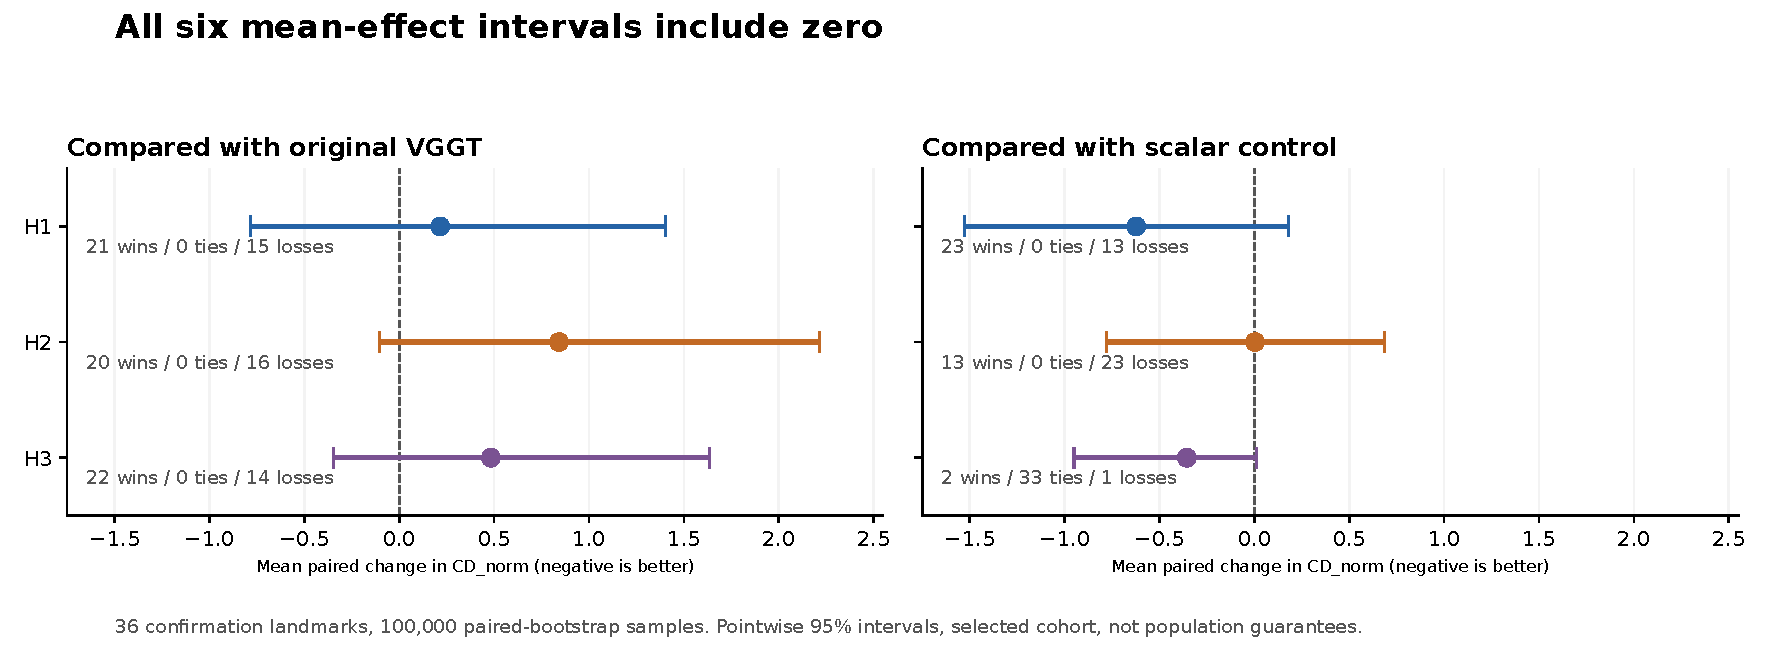
\includegraphics[width=\textwidth]{figures/extended_paired_effects.pdf}
\caption{Mean paired differences and pointwise 95\% landmark-bootstrap intervals against both references. The zero line denotes no mean change. H1 has the most favorable mean against the scalar, while the original model retains the lowest cohort mean error.}
\Description{Two panels show H1, H2, and H3 mean differences and bootstrap intervals against original VGGT and scalar steering. Every interval crosses zero.}
\label{fig:bootstrap}
\end{figure*}

H1's scalar-relative advantage survives every single-landmark omission, but the original-model comparison is sensitive to Pal\'acio Nereu Ramos. Removing that case changes H1's mean difference from $+0.2164$ to $-0.1884$. H2 and H3 remain worse than the original mean after every possible single omission. All 36 landmarks remain in the official scores. Omission is an influence diagnostic, not a revised result.

\paragraph{Exploratory feature search.}
We examine 28 primary continuous-feature associations using Spearman rank correlations and 18 categorical associations using rank-based permutation omnibus tests. Features include physical extent, variable strength coefficients, relative update magnitude, executed anchor, region, and building type. The 46 tests are pooled for Benjamini--Hochberg and Holm correction. None survives either global correction at 0.05. The smallest global BH $q$ is 0.09476. These analyses use the already-frozen confirmation outputs and do not fit a new selection rule.

The strongest categorical pattern is region for H1 relative to the scalar (raw $p=0.00206$, global $q=0.09476$). It passes correction within the smaller 18-test categorical family ($q=0.03708$), but not across the combined search. The corresponding original-model comparison has $p=0.41068$. North America has four scalar-relative wins from four landmarks and South Asia five from five. These small, overlapping geographic and architectural groups cannot identify a causal regional effect.

The strongest continuous hints are H3 relative-update magnitude versus its original-model difference ($\rho=+0.445$, raw $p=0.00672$, global $q=0.15456$), and H2 coefficient spread versus its scalar-relative difference ($\rho=-0.411$, raw $p=0.01412$, global $q=0.16238$). Positive associations indicate larger features accompany worse effects. Negative associations indicate better effects. Both retain their sign after each single-landmark omission, but neither establishes a usable predictor. For H3, 33 predictions duplicate the scalar, so the association mostly describes scalar behavior. For H2, 21 of 36 coefficient ratios tie at four. Average ranks handle those ties. The independently chosen base strengths also confound weighting with step magnitude.

Constant diagnostics were excluded. Every selected run accepted 24 layers, clipping counts were zero, and H1's mean relative update was essentially fixed at 0.02. View count is 50 for 35 landmarks and 26 for one, so it was not treated as an informative continuous predictor. Original error versus improvement shares an error term algebraically and is not evidence for a difficulty-based selector. Some H3--scalar bootstrap correlation samples contain only ties and have undefined correlation. Stored correlation intervals condition on defined samples. Additional log-ratio sensitivity checks provide no corrected discoveries.

\paragraph{Complementary successes.}
At least one hypothesis beats the original on 28 of 36 landmarks. All three beat it on 14 and none on eight. At least one beats both controls on 19 landmarks, while none of the landmarks is improved over both controls by all three methods. These counts identify complementary outcomes after observing ground truth. They do not measure the accuracy of an inference-time selector, and choosing the best observed method for each landmark would leak confirmation outcomes.

\subsection{Verified Reconstruction Examples}
\label{sec:qualitative-summary}
The exported confirmation examples are Herald Square for H1, Itmad-Ud-Daulah's Tomb for H2, and Marine Corps War Memorial for H3. Within each hypothesis, the case is selected post hoc as the largest percentage improvement over the original among landmarks that improve over both controls. They demonstrate possible gains, not typical performance. Table~\ref{tab:qualitative-cases} gives full-cloud numerical scores, and Appendix~\ref{app:qualitative} displays the reconstructions.

The nine re-exported conditions (original, scalar, and selected rule for each case) reproduce their recorded prediction hashes and metrics. Matched images, masks, and frozen settings are retained. Each displayed pair uses the same camera, point size, and framing, with real sampled geometry and no geometric smoothing. The H3 main view uses an explicitly shared scene crop because distant outliers otherwise dominate the framing. Its wide view is retained in the project. Crop selection does not change the full-cloud evaluation. These are whole-landmark comparisons, not separately scored anchor regions.

\begin{table*}[t]
\caption{Post-hoc qualitative cases. Scores are whole-landmark normalized Chamfer error, lower is better. Reductions are percentages for each selected landmark and do not replace the 36-landmark results.}
\label{tab:qualitative-cases}
\centering
\small
\begin{tabular}{lllrrrrr}
\toprule
Rule & Landmark & Anchor & Original & Scalar & Rule & \multicolumn{2}{c}{Reduction vs (\%)}\\
 & & & & & & Original & Scalar\\
\midrule
H1 & Herald Square & facade & 6.9134 & 6.5884 & 5.1401 & 25.65 & 21.98\\
H2 & Itmad-Ud-Daulah's Tomb & railing & 17.7941 & 23.6269 & 15.1476 & 14.87 & 35.89\\
H3 & Marine Corps War Memorial & statue & 31.6116 & 36.4341 & 28.0207 & 11.36 & 23.09\\
\bottomrule
\end{tabular}
\end{table*}
